\begin{figure}

\centering

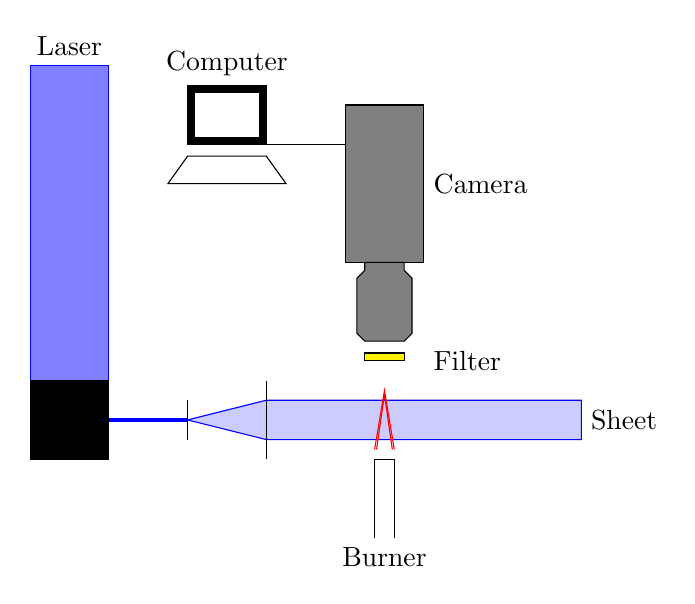
\begin{tikzpicture}

% Laser
\filldraw [fill=blue!50!white, draw=blue] ( 0, 5 ) rectangle ++( 1, -4 );
\filldraw [black] ( 0, 1 ) rectangle ++( 1, -1 );

% Beam
\draw [very thick, blue] ( 1, 0.5 ) -- ++( 1, 0 );
\draw [draw=blue,fill=blue!20!white] ( 2, 0.5 ) -- ++( 1, 0.25 ) -- ++( 4, 0 ) -- ++( 0, -0.5 ) -- ++( -4, 0 ) -- cycle;

% Lenses
\draw ( 2, 0.25 ) -- ++( 0, 0.5 );
\draw ( 3, 0 ) -- ++( 0, 1 );

% Laminar burner
\draw ( 4.375, -1 ) -- ++( 0, 1 ) -- ++( 0.25, 0 ) -- ++( 0, -1 );

% Flame
\draw [red] ( 4.375, 0.125 ) -- ++( 0.125, 0.75 ) -- ++( 0.125, -0.75 );
\draw [red] ( 4.4, 0.125 ) -- ++( 0.1, 0.7 ) -- ++( 0.1, -0.7 );

% Camera
\filldraw [fill=black!50!white, draw=black] ( 4, 4.5 ) rectangle ++( 1, -2 );
\filldraw [fill=black!50!white, draw=black] ( 4.25, 2.5 ) -- ++( 0, -0.1 ) -- ++( -0.1, -0.1 ) -- ++( 0, -0.7 ) -- ++( 0.1, -0.1 ) -- ++( 0.5, 0 ) -- ++( 0.1, 0.1 ) -- ++( 0, 0.7 ) -- ++( -0.1, 0.1 ) -- ++ ( 0, 0.1 ) -- cycle;

% Filter
\filldraw [fill=yellow, draw=black] ( 4.25, 1.25 ) rectangle ++( 0.5, 0.1 );

% Computer
\filldraw [black] ( 2, 4 ) rectangle ++( 1, 0.75 );
\filldraw [white]( 2.1, 4.1 ) rectangle ++( 0.8, 0.55 );
\draw ( 2, 3.85 ) -- ++( 1, 0 ) -- ++( 0.25, -0.35 ) -- ++( -1.5, 0 ) -- cycle;

\draw ( 3, 4 ) -- ++( 1, 0 );

% Labels
\node at ( 0.5, 5 ) [above] {Laser};
\node at ( 2.5, 4.75 ) [above] {Computer};
\node at ( 5, 3.5 ) [right] {Camera};
\node at ( 5, 1.25 ) [right] {Filter};
\node at ( 4.5, -1 ) [below] {Burner};
\node at ( 7, 0.5 ) [right] {Sheet};

\end{tikzpicture}

\caption[Schematic of the excitation scan experiment]{The figure above shows the schematic of the excitation scan experiment. A collimating pair of lenses form the laser beam into a sheet focused over a laminar Bunsen burner. The fluorescence is imaged perpendicularly by an intensified camera synchronized to the laser pulse. A 3 mm GG 420 filter is used to reject elastic scattering.}

\label{fig:excitationScan}

\end{figure}

